\section{Methods}\label{methods}

Fully dense neural network (NN) architectures, such as the one shown in Figure~\ref{fig:nn-1}, perform a sequence of affine transformations, ${\bold z}_i \leftarrow \boldsymbol\theta_i {\bold x}^{(i)}$, followed by element-wise functional operations, $\sigma({\bold z}_i)$ to introduce non-linearity at each layer; that is, each layer stretches and distorts the underlying space.
\begin{figure}[htbp]
\begin{center}
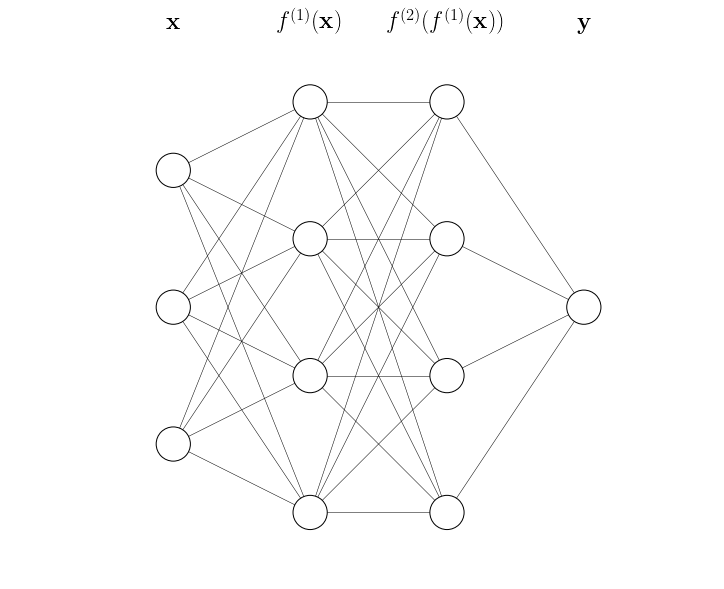
\includegraphics[width=0.4\textwidth]{fig/neural-network-01}
\caption{Schematic view of a fully dense neural network. Each sequence of affine and non-linear transformations are captured in the function, $f_i({\bold x}): {\bold x}^{(i+1)} \leftarrow \sigma(\boldsymbol\theta_i {\bold x}^{(i)})$}
\label{fig:nn-1}
\end{center}
\end{figure}

The resulting network,
\begin{equation}
	f(x) = \sigma(\boldsymbol\theta_n \sigma(\boldsymbol\theta_{n-1} \sigma(\ldots \boldsymbol\theta_2 \sigma(\boldsymbol\theta_1{\bold x}))))
	\label{eqn:nn analytical form}
\end{equation}
is an arbitrary function generator, but at present, the network weights $\boldsymbol\theta_i$ can not map back to analytic forms that capture and describe the underlying physics. There are, however, many such mappings through polynomial series expansions,
\begin{equation}
	f(x) = \sum_{n=0}^\infty a_n x^n
\end{equation}

The variable $\bold x$ in Equation~(\ref{eqn:nn analytical form}) represents a column vector containing $\boldsymbol n$ input elements, and thus, the output from each node is multplied by the respective weight before the application of the subsequent activation function, e.g.
\begin{equation}
	\bold z =
	\theta^{(1)} \begin{bmatrix}
				x_{1} \\
				x_{2} \\
				\vdots \\
				x_{n}
			\end{bmatrix}
	\Rightarrow \begin{bmatrix}
					\theta_{11} x_{1} + \theta_{12} x_{2} + \ldots \theta_{1n} x_{n} \\
					\theta_{21} x_{1} + \theta_{22} x_{2} + \ldots \theta_{2n} x_{n} \\
					\vdots \\
					\theta_{m1} x_{1} + \theta_{m2} x_{2} + \ldots \theta_{mn} x_{n} \\
				\end{bmatrix}
\end{equation}

and $\boldsymbol\sigma (\bold z)$ serves as the input of the next layer in the network, where $\bold z = (\boldsymbol\theta^{(1)} \bold x)$. \\*

We hypothesize that the physics of a process can be extracted by fitting the polynomial expansions of known physical relationships to the polynomial coefficients of a polynomial series expansion of Equation~(\ref{eqn:nn analytical form}). \\
\\*



%Beginning of softmax derivation 1/7
For example, consider the Softmax activation function which is given in Equation (???)

\begin{equation}
	\sigma(\bold z)_i =
	\frac{e^{z_i}}{\sum\limits_{j=1}^k e^{z_j}}
\end{equation}

The goal is to obtain a activation generating function for the chosen activation function in the neural network.

The partion function, $\bold Z$, is defined below as
\begin{equation}
	\bold Z = \sum\limits_{j=1}^k e^{z_j}
\end{equation}
The series representation for the exponential is given by the following
\begin{equation}
	e^{z_{i}} = \sum_{k=0}^{\infty}\frac{1}{k!} z_{i}^{k}
\end{equation}
Therefore
\begin{equation}
	\sigma(\bold z)_i =
	\sum\limits_{k=0}^{\infty} \alpha_{k}z_{i}^{k}
\end{equation}
Where $\alpha_k = \frac{1}{{\bold Z}k!}$ is the generating function for the Softmax
%End of softmax derivation 1/7


The ReLU (rectified linear units) function is another commonly used activation function and is given below in Equation~(\ref{eqn:ReLU}):
\begin{equation}
	f(x) =
	\begin{cases}
		x, & \text{if}\ x > 0 \\
		0, & \text{otherwise}
	\end{cases}
	\label{eqn:ReLU}
\end{equation}

The generating function for the ReLU is given in Equation~(\ref{eqn: ReLU generating function}) and it is dependent on both the input variables and the network weights.
\begin{equation}
	\alpha_n =
		\begin{cases}
			1 & \bold z > 0 \\
			0 & \text{otherwise}
		\end{cases}
	\label{eqn: ReLU generating function}
\end{equation}

Similarly, the linear generating function is given in Equation~(\ref{eqn: linear generating function}) but it is only dependent upon $\bold n$.
\begin{equation}
	\alpha_n =
		\begin{cases}
			1 & \bold n = 1 \\
			0 & \text{otherwise}
		\end{cases}
	\label{eqn: linear generating function}
\end{equation}

Although ReLU (rectified linear units) have become a more common activation function, its discontinuity at $x = 0$ requires an infinite series to fully capture the behavior at this transition.

However, the softplus function,

%Beginning of new Softplus Derivation 1/7
%The Softplus activation function is similar to the ReLU activation function, but unlike the ReLU, the first derivative of the Softplus is continuous. As will be discussed later, the Softplus can be modified such that it can be forced to converge to the ReLU.
\begin{align*}
	f(x) & = log(1+e^x)\\
	& = \frac{1}{\alpha}log(1+e^{\alpha x}), \quad \alpha > 0 \\
	& = \frac{1}{\alpha}log(z), \quad z = 1 + e^{\alpha x} \\
	& = \frac{1}{\alpha}\sum\limits_{k=1}^\infty
	\frac{1}{k}\left(\frac{z-1}{z}\right)^k \\
	& = \frac{1}{\alpha}\sum\limits_{k=1}^\infty
	\frac{1}{k}(z-1)^{k} z^{-k} \\
	& = \frac{1}{\alpha}\sum\limits_{k=1}^\infty
	\frac{1}{k} e^{\alpha x k} (1 + e^{\alpha x})^{k} \\
	& = \frac{1}{\alpha}\sum\limits_{k=1}^\infty
	\frac{1}{k} \left(\sum\limits_{m=0}^\infty
	\frac{\alpha^{m} x^{m}}{m!}\right)^k \left(1 + \sum\limits_{n=0}^{k} \frac{\alpha^{n} x^{n}}{n!}\right)^{-k}
\end{align*}

From Gradshteyn and Ryzhik - 0.314 Power series raised to powers.
\begin{equation}
	\left(\sum\limits_{k=0}^{\infty}a_{k}x^{k}\right)^{n} = \sum\limits_{k=0}^{\infty}c_{k}x^{k} \\
	\label{eqn:power series raised to powers}
\end{equation}
where
\begin{align*}
	c_{0} = a_{0}^{n}, \quad c_{m} = \frac{1}{ma_{0}}\sum\limits_{k=0}^{\infty}c_{k}x^{k}
\end{align*}

And therefore it can be seen that

\begin{align*}
	c_{0} = \frac{\alpha^{0}}{0!}=1, \quad c_{l} = \frac{1}{l}\sum\limits_{j=1}^{l}(jk-l+j)\frac{\alpha^{l}}{l!}c_{l-j}
\end{align*}

\begin{align*}
	& = \frac{1}{\alpha}\sum\limits_{k=1}^{\infty}\frac{1}{k}\sum\limits_{m=0}^{\infty}c_{m}x^{m}\left( 1+\sum\limits_{n=0}^{\infty}\frac{\alpha^{n}x^{n}}{n!}\right)^{-k} \\
\end{align*}

From Gradshteyn and Ryzhik - 1.1 Power of Binomials, 1.111 Power Series
\begin{equation}
	(a+x)^n = \sum\limits_{k=0}^{n}{n \choose k}x^k a^{n-k}
\end{equation}

And similarly

\begin{align*}
	& = \frac{1}{\alpha}\sum\limits_{k=1}^{\infty}\frac{1}{k}\sum\limits_{m=0}^{\infty}c_mx^m
	\left[ \sum\limits_{i=0}^{k}{k \choose i} \left( \sum\limits_{n=0}^{\infty}\frac{\alpha^nx^n}{n!} \right)^{i} \right]^{-1}
\end{align*}

Once again the substitution for a power series raised to a power is applied.

\begin{align*}
	d_{0} = 1, \quad d_{l}=\frac{1}{l}\sum\limits_{j=1}^{l}(ji-l+j)\frac{\alpha^{l}}{l!}d_{l-j}
\end{align*}

\begin{align*}
	& = \frac{1}{\alpha}\sum\limits_{k=1}^{\infty}\frac{1}{k}\left[ \frac{\sum\limits_{m=0}^{\infty}c_{m}x^{m}}{\sum\limits_{i=0}^{k}\frac{1}{{k \choose i}}\sum\limits_{n=0}^{\infty}d_{n}x^{n}} \right]
\end{align*}

After some rearranging of term, the result is given below.

\begin{align*}
	& = \frac{1}{\alpha}\sum\limits_{k=1}^{\infty}\frac{1}{k}\left[ \frac{\sum\limits_{m=0}^{\infty}c_{m}x^{m}}{\sum\limits_{n=0}^{\infty}\sum\limits_{i=0}^{k}\frac{1}{{k \choose i}}d_{n}x^{n}} \right] \\
\end{align*}

And therefore the following is obtained.
\begin{align*}
	& = \frac{1}{\alpha}\sum\limits_{k=1}^{\infty}\frac{1}{k}\left[ \frac{\sum\limits_{m=0}^{\infty}c_{m}x^{m}}{\sum\limits_{n=0}^{\infty}d_{n}'x^{n}} \right]
\end{align*}

Where
\begin{align*}
 	d_{n}' & = \sum\limits_{i=0}^{k}\frac{1}{{k \choose i}}d_{n}
\end{align*}

From Gradshteyn and Ryzhik - 0.313 Division of power series.

\begin{equation}
	\frac{\sum\limits_{k=0}^{\infty}b_k x^k}{\sum\limits_{k=0}^{\infty}a_k x^k}
	= \frac{1}{a_0}\sum\limits_{k=0}^{\infty}c_kx^k
\end{equation}

where

\begin{equation}
	c_n + \frac{1}{a_0}\sum\limits_{k=1}^n c_{n-k}a_k - b_n = 0
\end{equation}

And therefore

\begin{align*}
	b_{m} = \sum\limits_{j=1}^{m}c_{m}-b_{m-j}d_{j}
\end{align*}

\begin{align*}
	& = \frac{1}{\alpha}\sum\limits_{k=1}^{\infty}\frac{1}{k}\sum\limits_{n=0}^{\infty}b_{n}x^{n} \\
	& = \sum\limits_{n=0}^{\infty}\sum\limits_{k=1}^{\infty}\frac{b_{n}}{\alpha k}x^{n}=\frac{1}{\alpha}log(1+e^{\alpha x})
\end{align*}

where $\sum\limits_{k=1}^{\infty}\frac{b_{n}}{\alpha k}$ is the generating function for the softplus
%End of new softplus derivation 1/7

%\begin{equation}
%	f(x) = log(1+e^x)
%\end{equation}
%
%The series expansion for the exponential
%\begin{equation}
%	e^x = \sum_{k=0}^\infty \frac{x^k}{k!}
%\end{equation}
%where, $a_k = \frac{1}{k!}$, can be expressed as
%\begin{equation}
%	e^x = \sum_{k=0}^\infty x^k a_k
%\end{equation}
%
%A similar series expansion for the logarithm
%\begin{equation}
%	log(1+x) = \sum_{n=1}^\infty (-1)^{n+1} \frac{x^n}{n}
%\end{equation}
%where, $x = e^x$,
%allows for the softplus function to be represented as
%\begin{equation}
%	f(x) = \sum_{n=1}^\infty \frac{(-1)^{n+1}}{n} (\sum_{k=0}^\infty x^k a_k)^n
%\end{equation}
%
%If the expansion of $e^x$ is performed, then it can be seen that
%\begin{equation}
%	(\sum_{k=0}^\infty x^k a_k)^n = (a_0+x(a_1+x(a_2+xa_3...)))^n
%\end{equation}

%Beginning of old softplus derivation and could probably be deleted
%However, the softplus function,
%
%\begin{equation}
%	f(x) = log(1+e^x)
%\end{equation}
%
%The series expansion for the exponential
%\begin{equation}
%	e^x = \sum_{k=0}^\infty \frac{x^k}{k!}
%\end{equation}
%where, $a_k = \frac{1}{k!}$, can be expressed as
%\begin{equation}
%	e^x = \sum_{k=0}^\infty x^k a_k
%\end{equation}
%
%A similar series expansion for the logarithm
%\begin{equation}
%	log(1+x) = \sum_{n=1}^\infty (-1)^{n+1} \frac{x^n}{n}
%\end{equation}
%where, $x = e^x$,
%allows for the softplus function to be represented as
%\begin{equation}
%	f(x) = \sum_{n=1}^\infty \frac{(-1)^{n+1}}{n} 				(\sum_{k=0}^\infty x^k a_k)^n
%\end{equation}
%
%If the expansion of $e^x$ is performed, then it can be seen that
%\begin{equation}
%	(\sum_{k=0}^\infty x^k a_k)^n = 								(a_0+x(a_1+x(a_2+xa_3...)))^n
%\end{equation}
%
%Using the binomial theorem
%\begin{equation}
%	(a+b)^n = \sum_{m=0}^{n} \binom{n}{m} a^{n-m} b^m
%\end{equation}
%where, $a=a_0$ and $b=(x(a_1+x(a_2+xa_3...)))^n$, the series expansion of the exponential can be represented as
%\begin{equation}
%	(\sum_{k=0}^\infty x^k a_k)^n = \sum_{m=0}^{n} 				\binom{n}{m} a_0^{n-m} (a_1+x(a_2+xa_3...))^n x^n
%\end{equation}
%
%Continuing with this approach, it can be seen that ...
%End of old softplus derivation


{\color{red}
The element-wise exponent is used repeatedly in both the constitutive relation and neural network expansions. For the product of two matrices, $A: A \in \mathbb{R}^{m \times n}$ and $B: B \in \mathbb{R}^{n \times q}$, the element-wise exponent results in an expanded basis that explicitly includes the cross terms from ${\bf A}$ and ${\bf B}$.

\begin{subequations}
\begin{align}
        \left( AB \right)^{\circ p} &= \he[\left( \densematrix{a}{m}{n} \densematrix{b}{n}{q} \right)]{p} \nonumber \\
            &= \begin{pmatrix}
                {\bf a}_{1k}{\bf b}_{k1}  & {\bf a}_{1k}{\bf b}_{k2}    & \cdots    & {\bf a}_{1k}{\bf b}_{kq}   \\
                {\bf a}_{2k}{\bf b}_{k1}  & {\bf a}_{2k}{\bf b}_{k2}    &           & \vdots \\
                \vdots                    &                             & \ddots    &          \\
                {\bf a}_{mk}{\bf b}_{k1}  & \cdots                      &           & {\bf a}_{mk}{\bf b}_{kq}
            \end{pmatrix}^{\circ p} \nonumber \\
            &= \begin{pmatrix}
                ({\bf a}_{1k}{\bf b}_{k1})^{p}  & ({\bf a}_{1k}{\bf b}_{k2})^{p}    & \cdots    & ({\bf a}_{1k}{\bf b}_{kq})^{p}   \\
                ({\bf a}_{2k}{\bf b}_{k1})^{p}  & ({\bf a}_{2k}{\bf b}_{k2})^{p}    &           & \vdots \\
                \vdots                          &                                   & \ddots           &          \\
                ({\bf a}_{mk}{\bf b}_{k1})^{p}  & \cdots                            &           & ({\bf a}_{mk}{\bf b}_{kq})^{p}
            \end{pmatrix} \label{eqn:hadmard exponent matrix} \\[3ex]
        ({\bf a}_{ik}{\bf b}_{kj})^{p} &= (a_{i1}b_{1j} + a_{i2}b_{2j} + \cdots + a_{in}b_{nj})^p \nonumber \\
            &= \sum_{k1 + k2 + \cdots + k_n = p} \binom{p}{k_1, k_2, \ldots, k_n} \prod_{m=1}^n (a_{im}b_{mj})^{k_m} \nonumber \\
            &= \sum_{\| {\bf k} \|_1 = p} \binom{p}{k_1, k_2, \ldots, k_n} \prod_{m=1}^n (a_{im}b_{mj})^{k_m} \\%
    \label{eqn:hadamard exponent vector}
\end{align}
\label{eqn:nondistributive hadamard}
\end{subequations}
where summation over a repeated index is assumed. That is, Equation~\ref{eqn:hadamard exponent vector} is the expansion of the element-wise exponent of a vector product, $({\bf a}{\bf b})\he{p} = ({\bf a}{\bf b})^p \ne \he[{\bf a}]{p}\he[{\bf b}]{p}$.
}

% %%%%%%%%%%%%%%%%%%%%%%%%%%%%%%%%%%%%%%%%%%%%%%%%%%%%%%%%%%%%%%%%%%%%%%%%%%%%
The analytical form, combining Equations~(\ref{eqn:nn analytical form}) and (\ref{eqn:sigmoid zeta expansion}), the estimated output of a two-layer NN can be written as an expansion:

\begin{eqnarray}
	{\bold y}_1 & = & \sum_{k=0}^\infty a_k (\boldsymbol\theta_1^T {\bold x})\he{k} \nonumber \\
	{\bold y}_2 & = & \sum_{k=0}^\infty b_k (\boldsymbol\theta_2^T {\bold y}_1)\he{k} \nonumber \\
		& = & b_0 {\bold 1} + \nonumber\\
		&   & + b_1 (\tilde a_0 +%
					(\tilde a_1 + %
						(\tilde a_2 + %
							(\tilde a_3 + %
								(\ldots) \tilde {\bold x} )%
							\tilde {\bold x} )%
						\tilde {\bold x} )%
					\tilde {\bold x}) \nonumber \\
		&   & + b_2 (\tilde a_0 +%
					(\tilde a_1 + %
						(\tilde a_2 + %
							(\tilde a_3 + %
								(\ldots) \tilde {\bold x} )%
							\tilde {\bold x} )%
						\tilde {\bold x} )%
					\tilde {\bold x})^2 \nonumber \\
		&   & \vdots \nonumber \\
		&   & + b_k (\tilde a_0 +%
					(\tilde a_1 + %
						(\tilde a_2 + %
							(\tilde a_3 + %
								(\ldots) \tilde {\bold x} )%
							\tilde {\bold x} )%
						\tilde {\bold x} )%
					\tilde {\bold x})^k \nonumber \\
		&   & \vdots
\end{eqnarray}
\noindent where $\tilde a_i = \boldsymbol\theta_2^T a_i$ and $\tilde{\bold x} = \boldsymbol\theta_1^T {\bold x}$. All $\boldsymbol\theta_i$, ${\bold x}$, and ${\bold y}$ are augmented to include the bias, ${\bold b}_i$, that is,
\begin{eqnarray}
	{\bold x}&:& {\bold x} \leftarrow \begin{pmatrix}
								1 \\
								{\bold x}
							\end{pmatrix} = \begin{pmatrix}
											1 \\
											x_0 \\
											x_1 \\
											\vdots \\
											x_n
										\end{pmatrix}\\
	{\bold y}&:& {\bold y} \leftarrow \begin{pmatrix}
								1 \\
								{\bold y}
							\end{pmatrix} \\
	\boldsymbol\theta_i&:& \boldsymbol\theta_i \leftarrow \begin{pmatrix} {\bold b}_i & \boldsymbol\theta_i \end{pmatrix}
\end{eqnarray}

The element-wise exponent operator, ${\bf x}\he{m} = (x_1^m\ x_2^m\ \cdots\ x_n^m)^T$, raises each element of a vector or matrix to the specified power, $m$.

From Equation~(\ref{eqn:sigmoid zeta expansion}), $a_i  = 0\ \text{for}\ i = 2, 4, 6, \ldots$, and therefore,
\begin{align}
	{\bold y}_1 =& \sum_{k=0}^\infty a_k (\boldsymbol\theta_1^T {\bold x})\he{k} \nonumber \\
	{\bold y}_2 =& \sum_{k=0}^\infty b_k (\boldsymbol\theta_2^T {\bold y}_1)\he{k} \nonumber \\
		=& b_0 {\bold 1} + \nonumber\\
		 &+ b_1 (\tilde a_0 +%
					(\tilde a_1 + %
						(\tilde a_3 + %
							(\tilde a_5 + %
								(\ldots) \tilde {\bold x}\he{2} )%
							\tilde {\bold x}\he{2} )%
						\tilde {\bold x}\he{2} )%
					\tilde {\bold x}) \nonumber \\
		&+ b_2 (\tilde a_0 +%
					(\tilde a_1 + %
						(\tilde a_3 + %
							(\tilde a_5 + %
								(\ldots) \tilde {\bold x}\he{2} )%
							\tilde {\bold x}\he{2} )%
						\tilde {\bold x}\he{2} )%
					\tilde {\bold x})\he{2} \nonumber \\
		& \vdots \nonumber \\
		& + b_k (\tilde a_0 +%
					(\tilde a_1 + %
						(\tilde a_3 + %
							(\tilde a_5 + %
								(\ldots) \tilde {\bold x}\he{2} )%
							\tilde {\bold x}\he{2} )%
						\tilde {\bold x}\he{2} )%
					\tilde {\bold x})\he{k} \nonumber \\
		& \vdots \nonumber \\
	{\bold y}_2 = & \sum_{N=0}^\infty \sum_{k=0}^{N} \sum_{l=0}^{k} \sum_{m=0}^{l} \ldots %
		b_N %
		\binom{N}{k,l,m,\ldots} %
		\tilde a_0^k \tilde a_1^l \tilde a_3^m \ldots %
		\tilde {\bold x}\he{(N-k\ldots)} %
		({\tilde {\bold x}^2})\he{(N-k-l\ldots)} %
		({\tilde {\bold x}^2})\he{(N-k-l-m\ldots)} \nonumber \\
	 =& \sum_{N=0}^\infty \sum_{k=0}^{N} \sum_{l=0}^{k} \sum_{m=0}^{l} \ldots %
		b_N %
		\binom{N}{k,l,m,\ldots} %
		\tilde a_0^k \tilde a_1^l \tilde a_3^m \ldots %
		\tilde {\bold x}\he{(l+m+n+\ldots)} %
		({\tilde {\bold x}\he{2}})\he{(m+n+\ldots)} %
		({\tilde {\bold x}\he{2}})\he{(n+\ldots)}
	\label{eqn:ANN power series coefficient generating function}
\end{align}
\noindent where $k+l+m+n+\ldots = N$. Collecting coefficients and terms of power $k$,
\begin{equation*}
	{\bold y_2} =  \sum_{k=0}^\infty c_k \tilde{\bold x}\he{k}
\end{equation*}
\noindent that, having the same form as Equation~(\ref{eqn:sigmoid zeta expansion}) creates a sequential process for determining the coefficients of the power series expansion of each layer in an ANN. Importantly, the output layer in a ANN regression is a single node with a linear activation, so the final layer, $y_f$, working from the last hidden layer, ${\bold y}_n$, is simply,
\begin{equation}
	y_f = \boldsymbol\theta_n^T {\bold y}_n
\end{equation}


%If no reference, prove that the primal/dual is unique.
%Weidmann J. (1980) Linear operators and their adjoints. In: Linear Operators in Hilbert Spaces. Graduate Texts in Mathematics, vol 68. Springer, New York, NY
%Riesz representation theorem for proving that the dual is unique???
